


\documentclass[9pt,fleqn,a4paper]{article}

\usepackage[russian]{babel}
\usepackage[utf8]{inputenc}
\usepackage{amsmath}
\usepackage{amsfonts}
\usepackage{enumitem}
\usepackage{ntheorem}
\usepackage{tikz}
\usepackage{verbatim}
\usepackage{ amssymb}


\usepackage{mathtools}
\usepackage{subfigure}
\usepackage{cancel}
\def\multiset#1#2{\ensuremath{\left(\kern-.3em\left(\genfrac{}{}{0pt}{}{#1}{#2}\right)\kern-.3em\right)}}



\usepackage[left=2cm,right=2cm,top=2cm,bottom=2cm,bindingoffset=0cm]{geometry}
\renewcommand{\baselinestretch}{1.2}

\usepackage{graphicx}
\graphicspath{{}}
\DeclareGraphicsExtensions{.pdf,.png,.jpg}

\sloppy

\usetikzlibrary{arrows,shapes}

\tikzstyle{vertex}=[circle,fill=black,minimum size=3pt,inner sep=0pt]
\tikzstyle{edge} = [draw,thick,-]

\newtheorem*{definition}{Определение}
\newtheorem*{solution}{Решение}

\newenvironment{task}[2] {
	\noindent\fbox{\bf {#1} {#2}}
}{
}

\newcommand{\mytitle}[2] {
  \begin{center}
      \bf {#1} {#2}.
  \end{center}
}

\let\origenumerate\enumerate
\let\origendenumerate\endenumerate
\renewenvironment{enumerate}{\origenumerate[topsep = 0pt, noitemsep]}{\origendenumerate}


\begin{document}

	\begin{tabbing}
	\hspace{11cm} \= \= Щербаков Максим, 28 лет \\
	 \> Инженер-программист \\
	\> Санкт-Петербург, готов к командировкам \\
	\>  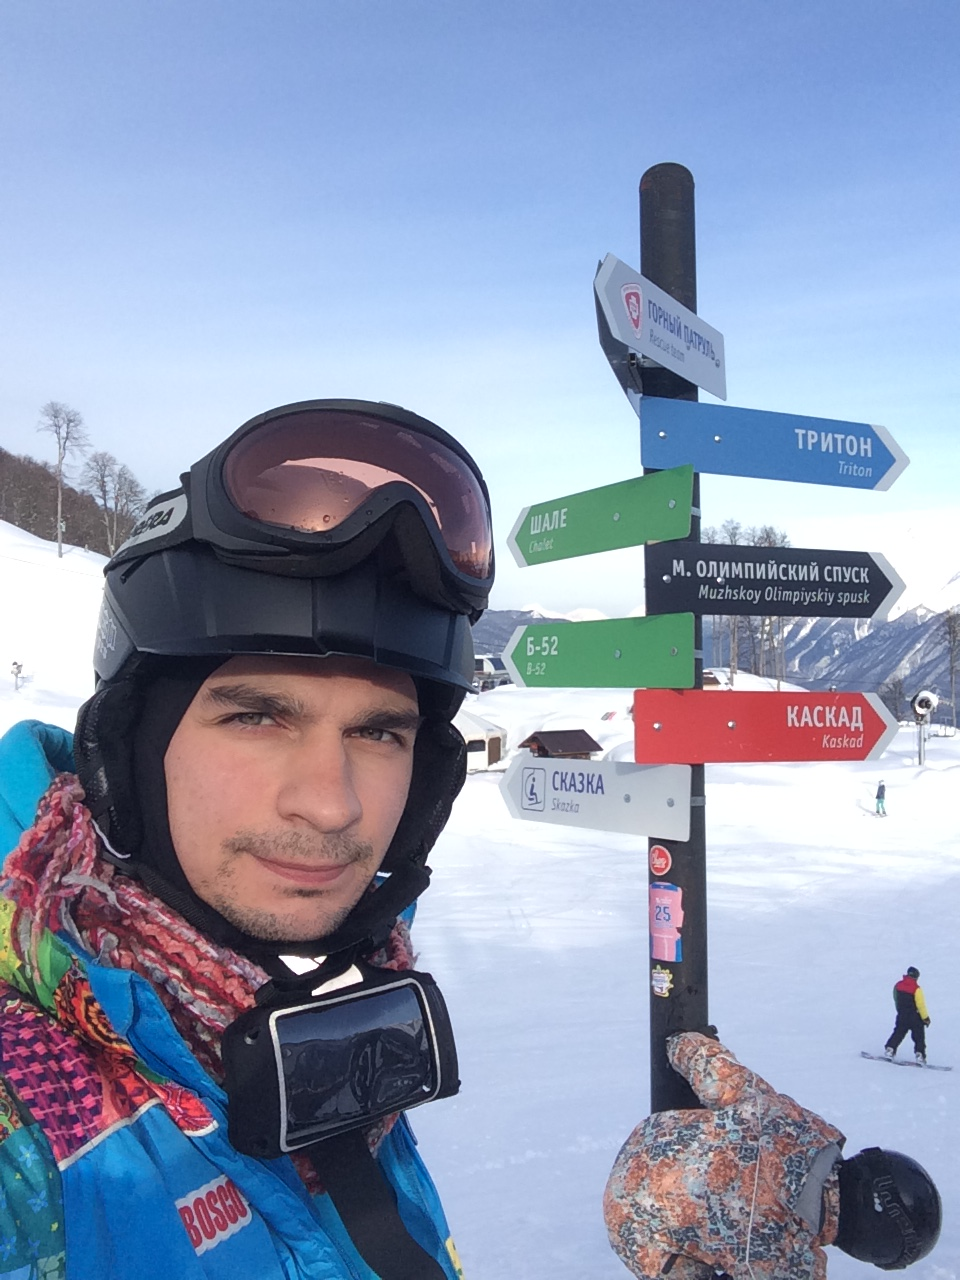
\includegraphics[width=4.5cm]{foto} \\
	\> +7 (950) 014-89-40  \\
	\> maxim.y.scherbakov@gmail.com — \\
	\> предпочитаемый способ связи

  	\end{tabbing}
	\hrule
	\vspace{1cm}




	\begin{center}
		{\large\bf C++ developer}
	\end{center}	
	
	\noindentИнформационные технологии, интернет, телеком \\
	Программирование, Разработка \\
	Занятость: полная занятость \\

	\noindentГрафик работы: гибкий график, полный день \\

	\begin{center}
		{\large\bf Опыт работы 5 лет 4 месяца}
	\end{center}	
	
	\noindentИюль 2014 — по настоящее время\\
5 лет 4 месяца \\
	Вооруженные силы РФ mil.ru \\
	Инженер-программист \\
Разработка программных модулей для обработки цифровых сигналов. \\
Поддержка специального программного обеспечения.  \\
Выполнение обязанностей оператора. \\

	\begin{center}
		{\large\bf Ключевые навыки}
	\end{center}	
	
	\noindent C/C++, Git, Microsoft Visual Studio, Linux, Windows, JetBrains CLion, Алгоритмы и структуры данных,  
        Работа в команде, Коммуникабельность, Грамотная речь, Английский язык, Ответственность \\

	\begin{center}
		{\large\bf Обо мне}
	\end{center}	

Привык ставить цели и добиваться их. Окончил один из самых престижных физико-математических лицеев в России - очень важный этап моей жизни, здесь я научился работать. Окончил с медалью Минобороны элитный военный ВУЗ - Военную инженерно-космическую академию им. Можайского - здесь научился дисциплине, преодолению трудностей, забыл что значит "невозможно". Стал офицером Вооруженных Сил РФ. И при этом инженером-программистом. Настоящая цель хорошо обдумана: развиваться дальше в любимой области - программировании. Именно поэтому решил не продлевать свой военный контракт, а поступил в Computer Science Center и сейчас ищу команду, в которой я буду расти. Основной инструмент - C++, есть опыт работы именно на нем, но открыт и к другим языкам (Java, C\#) также сталкивался с Python, R, Javascript, HTML, CSS, MySQL. Знаком с Git.

В мае 2019 в составе команды JetBrains Research (https://research.jetbrains.org/), принимал участие и победил в AI Driving Olympics (https://www.icra2019.org/competitions/ai-driving-olympics-ai-do) - соревнованиях по автономному управлению роботами.
(AI technologies, Python, Docker, C++),

Профиль на GitHub: https://github.com/Bnaich

	\begin{center}
		{\large\bf Высшее образование}
	\end{center}

\begin{tabbing}
2021
	\hspace{5cm} \= \= Computer Science Center \\
	 \> Software development \\
\\
2017
	\hspace{5cm} \= \= Российская академия народного хозяйства и государственной службы\\ \> при Президенте РФ, Москва
Юридический факультет, \\ \> Международное право \\
\\
2014
	\hspace{5cm} \= \= Военно-космическая академия им. А.Ф. Можайского, Санкт-Петербург \\
\> Факультет сбора и обработки информации, \\ \> Информационные системы и технологии
 \\
\end{tabbing}

	\begin{center}
		{\large\bf Знание языков}
	\end{center}	
	
	\noindentРусский — Родной \\
	Английский — B2 — Средне-продвинутый \\
	
	
\end{document}